\documentclass[12pt]{article}
\usepackage{graphicx}
\usepackage{gensymb}
\usepackage[none]{hyphenat}
\usepackage{graphicx}
\usepackage{listings}
\usepackage[english]{babel}
\usepackage{graphicx}
\usepackage{caption}
\usepackage{hyperref}
\usepackage{booktabs}
\usepackage{array}
\usepackage{amsmath}
\usepackage{listings}
\usepackage{multirow}
\usepackage{blindtext}
\usepackage{capt-of}
\usepackage{circuitikz}
\usepackage{./karnaugh-map}
\usetikzlibrary{shapes.geometric}
\title{Implementation of 4x1 mux using Arm(VAMAN)}
\date{March 2023}
\author{Marikundam Harshitha\\marikundamdec@gmail.com\\FWC22120\\IIT Hyderabad-Future Wireless Communication Assignment - 4}
\lstset{
	frame=single'
	breaklines=true
}
\newcommand{\mydet}[1]{\ensuremath{\begin{vmatrix}#1\end{vmatrix}}}
\providecommand{\brak}[1]{\ensuremath{\left(#1\right)}}
\providecommand{\norm}[1]{\left\lvert#1\right\rVert}
\newcommand{\solution}{\noindent \textbf{Solution: }}
\newcommand{\myvec}[1]{\ensuremath{\begin{pmatrix}#1\end{pmatrix}}}
\let\vec\mathbf

\begin{document}
\maketitle
\tableofcontents
\pagebreak

	 \section{Problem}
	 (GATE EC-2022)\\

Q.19. Consider the 2-bit multiplexer(MUX) shown in the figure.For output to be the XOR of R and S,the values for $ W,X,Y$ and $Z$ are ?\newline
\begin{figure}[h]
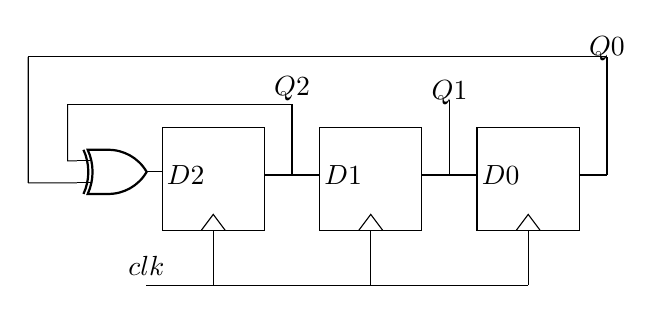
\begin{tikzpicture}
\ctikzset{                                   
logic ports=ieee,                   
logic ports/scale=0.5               
}                                    
\draw(-1.3,-0.56)node[xor port,anchor=out](x) {};  
%Drawing flip-flops
\draw (-1.3,-1.3) rectangle (0,0);
\draw(-1,-0.6) node{$D2$};
\draw(0.7,-1.3) rectangle (2,0);
\draw(1,-0.6) node{$D1$};
\draw(2.7,-1.3) rectangle (4,0);
\draw(3,-0.6) node{$D0$};
%connecting them
\draw(0,-0.6) -- (0.7,-0.6);
\draw(2,-0.6) -- (2.7,-0.6);
\draw(4,-0.6) -- (4.35,-0.6);
%drawing clk
\draw(-1.5,-2) node[above]{$clk$} -- (3.35,-2);
%connecting clk 
\draw(-0.65,-2) -- (-0.65,-1.3);
\draw(1.35,-2) -- (1.35,-1.3);
\draw(3.35,-2) -- (3.35,-1.3);
%drawing clk edges
\draw(-0.5,-1.3) -- (-0.65,-1.1) -- (-0.8,-1.3);
\draw(1.2,-1.3) -- (1.35,-1.1) -- (1.5,-1.3);
\draw(3.2,-1.3) -- (3.35,-1.1) -- (3.5,-1.3);
%drawing Q2,Q1,Q0
\draw(0.35,-0.6) --(0.35,0.3);
\draw(2.35,-0.6) --(2.35,0.35);
\draw(4.35,-0.6) --(4.35,0.9);
\draw(4.35,0.9) -- (-3,0.9);
\draw(0.35,0.3) -- (-2.5,0.3);
\draw(x.in 2) -|(-3,-0.7)to[short](-3,0.9);
\draw(x.in 1) -|(-2.5,-0.3)to[short](-2.5,0.3);
\draw(0.35,0.5)node{$Q2$};
\draw(2.35,0.45)node{$Q1$};
\draw(4.35,1)node{$Q0$};
\end{tikzpicture}

\caption{mux}
\label{fig:1}
\end{figure}
\begin{enumerate}
\item $W = 0, X = 0, Y = 1, Z = 1$
\item $W = 1, X = 0, Y = 1, Z = 0$
\item $W = 0, X = 1, Y = 1, Z = 0$
\item $W = 1, X = 1, Y = 0, Z = 0$
\end{enumerate}
\section{Introduction}
	The above diagram is a 4:1 multiplexer where $W, X, Y, Z$ are the inputs of the multiplexer and $A$ is the output of the multiplexer.$R , S$ are the select lines of the multiplexer,which means:\newline
\begin{enumerate}
\item For $R = 0,S = 0$,the first input line $W$ is selected.
\item For $R = 0,S = 1$,the second input line $X$ is selected.
\item For $R = 1,S = 0$,the third input line $Y$ is selected.
\item For $R = 1,S = 1$,the fourth input line $Z$ is selected.
\end{enumerate}
Therefore,the resultant output expression of the multiplexer is $R'S'W + R'SX + RS'Y + RSZ$.
\section{Components}
\begin{table}[h]
	\begin{tabular}{|p{3cm}|p{3cm}|p{3cm}|}
\hline                                        
\textbf{Symbol} & \textbf{Values} & \textbf{Description}\\                                          
\hline                                 
$\theta$ & 30$\degree{}$   & $\angle{BAD} = \angle{BAC}$ \\           
\hline                                    
a &  9 & $AB$ \\     
\hline                      
c & 5 & $AC$ \\
\hline                                     
		$\vec{e}_1$ & $\myvec{
			1\\
			0\\
			}$ & basis vector\\ 
\hline
\end{tabular}

\caption{contents}
\label{table 1}
\end{table}
	\pagebreak
\section{Hardware}
	\begin{enumerate}
\item Set the GPIO pins: 4,5,6,7,8,9 of Vaman as inputs.
\item Set the GPIO pin 10 of Vaman as output.
\item Read the input pins after connecting the Vcc and GND pins.
\item Verify the outputs using the truth table.
\end{enumerate}
\begin{table}[h]
\begin{center}
	\begin{tabular}{|p{2cm}|p{2cm}|p{2cm}|}
\hline
\multicolumn{3}{|c|}{Truth table}\\
\hline
R& S& A\\
\hline
0& 0& 0\\
\hline
0& 1& 1\\
\hline
1& 0& 1\\
\hline
1& 1& 0\\
\hline
\end{tabular}

\end{center}
\caption{truth table}
\label{table 2}
\end{table}
The K-map for this truth table will be a two variable K-map and it will be as follows:
\begin{figure}[h]
		\begin{center}
	\begin{karnaugh-map}[2][2][1][$R$][$S$]
		\minterms{1,2}
		\autoterms[0]
	\end{karnaugh-map}
	\end{center}	

\caption{k-map}
\label{fig2}
\end{figure}

So,the resultant expression of A is $A = R'S + RS'$.
\pagebreak
\section{Software}

The embedded code for the given circuit is \\
\lstinputlisting{src/main.c}
\end{document}
